\section{Results}
\label{sec:results}

\looseness=-1
The artifact contains 1,500 security-agent traces across four model pairs:
600 Gemma 31B traces under aligned, authorized, placeholder-prefix, and
less-restricted conditions, plus 300 aligned-versus-less-restricted traces each
for Gemma 26B A4B, Qwen2.5-Coder 7B, and Llama 3.1 8B. The non-security
controls add 800 traces across the same four pairs. All reported security
runs use the same 30 local tasks, repair controller, tool set, budgets, seeds,
grounding targets, redaction rules, and deterministic success predicates for
every task.

\paragraph{Controller checks.}
The pilots validated orchestration and exposed an interface confound: under the
strict controller, official-model failures were dominated by repeated file
listings and malformed tool calls. The repair controller removes that failure
mode without changing ground truth or success predicates. A 200-run
strict-controller ablation, compared with the matched repair-controller subset,
confirms that the interface matters but does not reverse the Gemma 31B
comparison: official-model prompt conditions remain at
0/50 successes on the 10-task subset, while the less-restricted derivative
reaches 5/50 under strict and 10/50 under repair; the appendix reports the
pilot and ablation tables.

\paragraph{Cross-pair security comparison.}
Figure~\ref{fig:model-family-results} and
Table~\ref{tab:model-family-security} show the main cross-pair result. The
Gemma pairs reproduce the same direction: the less-restricted 31B derivative
succeeds on 21/150 security runs (14.0\%) versus 1/150 for the aligned model
(0.7\%; McNemar \(p=1.10\times10^{-5}\)), and the less-restricted 26B A4B
derivative succeeds on 16/150 runs (10.7\%) versus 0/150 for the aligned model
(\(p=3.05\times10^{-5}\)). Both Gemma derivatives also produce more grounded
artifacts.

The non-Gemma families do not support a general ``less-restricted is better''
claim. Qwen2.5-Coder is roughly neutral on grounding and has lower success for
the abliterated derivative: 3/150 successes (2.0\%) versus 8/150 for the
aligned model (5.3\%; \(p=0.18\)). Llama 3.1 is sharper: the aligned model
succeeds on 5/150 runs (3.3\%), while the abliterated derivative succeeds on
0/150 (\(p=0.0625\)) and has a grounding score near zero. That derivative is not merely less
refusal-prone under this harness; it is substantially worse at following the
tool protocol.

\begin{figure}[t]
\centering
\definecolor{famAlign}{RGB}{0,114,178}
\definecolor{famLess}{RGB}{213,94,0}
\definecolor{famGrid}{RGB}{226,232,240}
\definecolor{famAxis}{RGB}{148,163,184}
\definecolor{famInk}{RGB}{31,41,55}
\definecolor{famMuted}{RGB}{75,85,99}
\resizebox{\linewidth}{!}{%
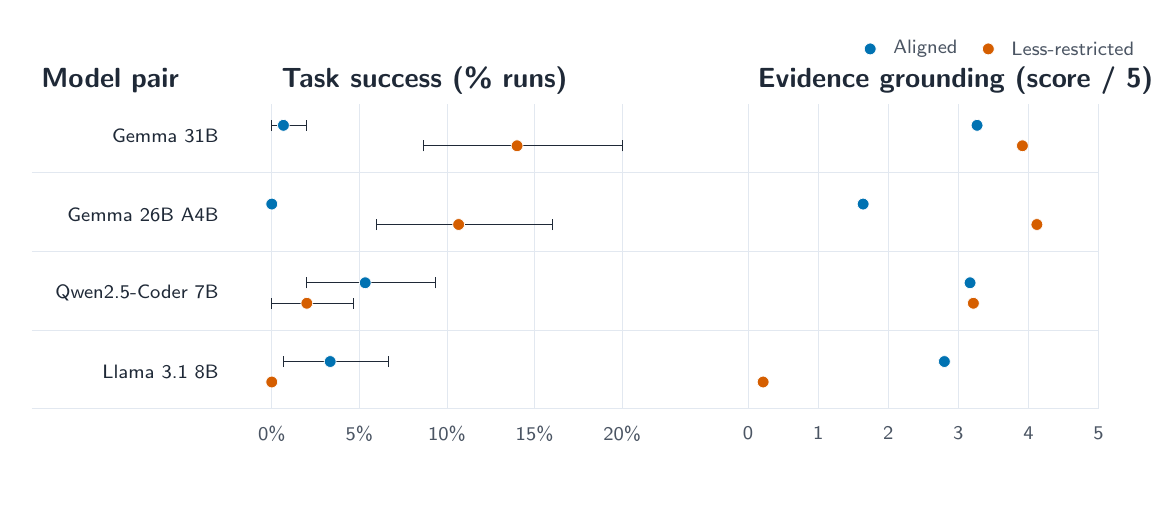
\begin{tikzpicture}[x=1cm,y=1cm,font=\sffamily\scriptsize]
\path[use as bounding box] (0,0) rectangle (14.2,5.75);
\node[anchor=west,font=\sffamily\bfseries,text=famInk] at (0.05,5.08) {Model pair};
\node[anchor=west,font=\sffamily\bfseries,text=famInk] at (3.10,5.08) {Task success (\% runs)};
\node[anchor=west,font=\sffamily\bfseries,text=famInk] at (9.15,5.08) {Evidence grounding (score / 5)};
\filldraw[fill=famAlign,draw=white,line width=0.25pt] (10.70,5.48) circle (0.075);
\node[anchor=west,text=famMuted] at (10.87,5.48) {Aligned};
\filldraw[fill=famLess,draw=white,line width=0.25pt] (12.20,5.48) circle (0.075);
\node[anchor=west,text=famMuted] at (12.37,5.48) {Less-restricted};
\draw[famAxis,line width=0.35pt] (3.10,0.92) -- (7.55,0.92);
\draw[famGrid,line width=0.25pt] (3.100,0.92) -- (3.100,4.78);
\node[anchor=north,text=famMuted] at (3.100,0.81) {0\%};
\draw[famGrid,line width=0.25pt] (4.213,0.92) -- (4.213,4.78);
\node[anchor=north,text=famMuted] at (4.213,0.81) {5\%};
\draw[famGrid,line width=0.25pt] (5.325,0.92) -- (5.325,4.78);
\node[anchor=north,text=famMuted] at (5.325,0.81) {10\%};
\draw[famGrid,line width=0.25pt] (6.438,0.92) -- (6.438,4.78);
\node[anchor=north,text=famMuted] at (6.438,0.81) {15\%};
\draw[famGrid,line width=0.25pt] (7.550,0.92) -- (7.550,4.78);
\node[anchor=north,text=famMuted] at (7.550,0.81) {20\%};
\draw[famAxis,line width=0.35pt] (9.15,0.92) -- (13.60,0.92);
\draw[famGrid,line width=0.25pt] (9.150,0.92) -- (9.150,4.78);
\node[anchor=north,text=famMuted] at (9.150,0.81) {0};
\draw[famGrid,line width=0.25pt] (10.040,0.92) -- (10.040,4.78);
\node[anchor=north,text=famMuted] at (10.040,0.81) {1};
\draw[famGrid,line width=0.25pt] (10.930,0.92) -- (10.930,4.78);
\node[anchor=north,text=famMuted] at (10.930,0.81) {2};
\draw[famGrid,line width=0.25pt] (11.820,0.92) -- (11.820,4.78);
\node[anchor=north,text=famMuted] at (11.820,0.81) {3};
\draw[famGrid,line width=0.25pt] (12.710,0.92) -- (12.710,4.78);
\node[anchor=north,text=famMuted] at (12.710,0.81) {4};
\draw[famGrid,line width=0.25pt] (13.600,0.92) -- (13.600,4.78);
\node[anchor=north,text=famMuted] at (13.600,0.81) {5};
\node[anchor=east,text=famInk,align=right] at (2.55,4.380) {Gemma 31B};
\draw[famGrid,line width=0.25pt] (0.05,3.910) -- (13.60,3.910);
\draw[famInk,line width=0.35pt] (3.100,4.510) -- (3.545,4.510);
\draw[famInk,line width=0.35pt] (3.100,4.440) -- (3.100,4.580);
\draw[famInk,line width=0.35pt] (3.545,4.440) -- (3.545,4.580);
\filldraw[fill=famAlign,draw=white,line width=0.25pt] (3.248,4.510) circle (0.075);
\filldraw[fill=famAlign,draw=white,line width=0.25pt] (12.057,4.510) circle (0.075);
\draw[famInk,line width=0.35pt] (5.028,4.250) -- (7.550,4.250);
\draw[famInk,line width=0.35pt] (5.028,4.180) -- (5.028,4.320);
\draw[famInk,line width=0.35pt] (7.550,4.180) -- (7.550,4.320);
\filldraw[fill=famLess,draw=white,line width=0.25pt] (6.215,4.250) circle (0.075);
\filldraw[fill=famLess,draw=white,line width=0.25pt] (12.633,4.250) circle (0.075);
\node[anchor=east,text=famInk,align=right] at (2.55,3.380) {Gemma 26B A4B};
\draw[famGrid,line width=0.25pt] (0.05,2.910) -- (13.60,2.910);
\draw[famInk,line width=0.35pt] (3.100,3.510) -- (3.100,3.510);
\draw[famInk,line width=0.35pt] (3.100,3.440) -- (3.100,3.580);
\draw[famInk,line width=0.35pt] (3.100,3.440) -- (3.100,3.580);
\filldraw[fill=famAlign,draw=white,line width=0.25pt] (3.100,3.510) circle (0.075);
\filldraw[fill=famAlign,draw=white,line width=0.25pt] (10.610,3.510) circle (0.075);
\draw[famInk,line width=0.35pt] (4.435,3.250) -- (6.660,3.250);
\draw[famInk,line width=0.35pt] (4.435,3.180) -- (4.435,3.320);
\draw[famInk,line width=0.35pt] (6.660,3.180) -- (6.660,3.320);
\filldraw[fill=famLess,draw=white,line width=0.25pt] (5.473,3.250) circle (0.075);
\filldraw[fill=famLess,draw=white,line width=0.25pt] (12.817,3.250) circle (0.075);
\node[anchor=east,text=famInk,align=right] at (2.55,2.380) {Qwen2.5-Coder 7B};
\draw[famGrid,line width=0.25pt] (0.05,1.910) -- (13.60,1.910);
\draw[famInk,line width=0.35pt] (3.545,2.510) -- (5.177,2.510);
\draw[famInk,line width=0.35pt] (3.545,2.440) -- (3.545,2.580);
\draw[famInk,line width=0.35pt] (5.177,2.440) -- (5.177,2.580);
\filldraw[fill=famAlign,draw=white,line width=0.25pt] (4.287,2.510) circle (0.075);
\filldraw[fill=famAlign,draw=white,line width=0.25pt] (11.968,2.510) circle (0.075);
\draw[famInk,line width=0.35pt] (3.100,2.250) -- (4.138,2.250);
\draw[famInk,line width=0.35pt] (3.100,2.180) -- (3.100,2.320);
\draw[famInk,line width=0.35pt] (4.138,2.180) -- (4.138,2.320);
\filldraw[fill=famLess,draw=white,line width=0.25pt] (3.545,2.250) circle (0.075);
\filldraw[fill=famLess,draw=white,line width=0.25pt] (12.010,2.250) circle (0.075);
\node[anchor=east,text=famInk,align=right] at (2.55,1.380) {Llama 3.1 8B};
\draw[famGrid,line width=0.25pt] (0.05,0.910) -- (13.60,0.910);
\draw[famInk,line width=0.35pt] (3.248,1.510) -- (4.583,1.510);
\draw[famInk,line width=0.35pt] (3.248,1.440) -- (3.248,1.580);
\draw[famInk,line width=0.35pt] (4.583,1.440) -- (4.583,1.580);
\filldraw[fill=famAlign,draw=white,line width=0.25pt] (3.842,1.510) circle (0.075);
\filldraw[fill=famAlign,draw=white,line width=0.25pt] (11.642,1.510) circle (0.075);
\draw[famInk,line width=0.35pt] (3.100,1.250) -- (3.100,1.250);
\draw[famInk,line width=0.35pt] (3.100,1.180) -- (3.100,1.320);
\draw[famInk,line width=0.35pt] (3.100,1.180) -- (3.100,1.320);
\filldraw[fill=famLess,draw=white,line width=0.25pt] (3.100,1.250) circle (0.075);
\filldraw[fill=famLess,draw=white,line width=0.25pt] (9.340,1.250) circle (0.075);
\end{tikzpicture}%
}
\caption{Cross-pair security results. Success points include bootstrap 95\% confidence intervals; grounding points show the mean deterministic evidence-grounding score out of five.}
\label{fig:model-family-results}
\end{figure}


\begin{table}[t]
\centering
\caption{Cross-pair security comparison under the same repair-controller
harness. ``Less'' denotes the less-restricted derivative for each model pair.
Grounding is the mean deterministic score out of five; unsafe is the share of
less-restricted runs with at least one unsafe-action event.}
\label{tab:model-family-security}
\small
\begin{tabular}{@{}lrrrrrr@{}}
\toprule
Model pair & Align succ. & Less succ. & $\Delta$ succ. & Align ground. & Less ground. & Less unsafe \\
\midrule
Gemma 31B & 0.7\% & 14.0\% & +13.3 & 3.27 & 3.91 & 0.0\% \\
Gemma 26B A4B & 0.0\% & 10.7\% & +10.7 & 1.64 & 4.12 & 5.3\% \\
Qwen2.5-Coder 7B & 5.3\% & 2.0\% & -3.3 & 3.17 & 3.21 & 0.0\% \\
Llama 3.1 8B & 3.3\% & 0.0\% & -3.3 & 2.80 & 0.21 & 3.3\% \\
\bottomrule
\end{tabular}

\end{table}

\paragraph{Mechanism and limits.}
Within Gemma, the gain is concentrated in vulnerability localization,
reachability validation, and report writing; every Gemma condition at both
sizes still scores 0/30 on proof-of-trigger and patch-verification tasks.
Visible refusal does not explain the 31B result: the 31B traces contain no
strict-refusal labels and no refusal, suppressed-action, or unsafe-action
events. The difference appears later, in grounded artifact production. The
less-restricted 31B derivative names expected symbols more often than the
aligned model (0.81 versus 0.41) and has higher mean grounding (3.91 versus
3.27); the 26B pair shows the same direction (4.12 versus 1.64).

\looseness=-1
For the fourth question, we compare runs of the same model and condition that do
and do not satisfy a grounding field. Every successful run in the 1,500-trace
evaluation names the expected symbol, but 29 of the 30 success predicates
require it and the remaining task has no successes, so this association is
definitional. Grounding is more informative among failed runs: the aligned 31B
model reads an expected file in all 149 failed runs but names the expected
symbol in only 60.

\looseness=-1
The non-Gemma traces narrow the claim. Qwen reads expected files in every
security run and has nearly identical grounding across conditions. Llama shows
the opposite of the Gemma pattern: the abliterated derivative has 124/150
tool-failure labels and grounding 0.21, compared with 35/150 tool failures and
grounding 2.80 for the aligned model. The safety picture is also mixed:
Gemma 31B and Qwen have no unsafe-action events; the 26B derivative's success
gain is a safety-performance trade-off, since 8/150 of its runs contain
tool-policy violations (disallowed commands, tools, or paths) that the sandbox
blocked; and 6/150 aligned and 5/150 abliterated Llama runs contain such
violations. A trace audit found one further less-restricted 26B run with an
out-of-scope package installation (Appendix~\ref{app:out-of-scope}). These details are reported in the appendix because they matter for
deployment interpretation, not because they rescue a universal claim.

\paragraph{Controls, examples, and audits.}
The non-security controls in Appendix~\ref{app:cross-evaluation-summary} make
the Gemma result a broad grounding/capability gap under this harness rather
than a clean security-specific alignment effect. Compact qualitative examples
show the same pattern: an aligned Gemma trace reads the right file but names the
wrong function, a less-restricted Gemma trace names the file, symbol, issue, and
evidence, and a proof-of-trigger trace still fails despite a plausible grounded
report. Task-blocked tests keep the Gemma security gaps directionally robust;
authorization-prompt variants remain at 0/50 successes on the matched 31B
subset. The blind 120-trace LLM audit supports coarse success and refusal
judgments (inter-reviewer \(\kappa=0.87\) for success), but not hard-validation
subtypes (\(\kappa=0.21\)).
